\documentclass[11pt, a4paper]{article}
\usepackage[utf8]{inputenc}
\usepackage[T1]{fontenc}
\usepackage[english]{babel}
\usepackage{geometry}
\usepackage{booktabs}
\usepackage{hyperref}
\usepackage{lmodern}
\usepackage{graphicx}
\usepackage[table]{xcolor} % Ajout pour la couleur des tableaux
\usepackage{pgfplots} % Ajout pour les graphiques
\pgfplotsset{compat=1.18} % Spécifier une version de compatibilité

% Couleurs personnalisées
\definecolor{lightgreen}{rgb}{0.85,1,0.85}
\definecolor{lightorange}{rgb}{1,0.9,0.8}
\definecolor{lightred}{rgb}{1,0.8,0.8}
\definecolor{vuln-critical}{rgb}{0.6,0,0}
\definecolor{vuln-high}{rgb}{1,0.5,0}
\definecolor{vuln-medium}{rgb}{0.8,0.8,0}
\definecolor{vuln-low}{rgb}{0.6,0.8,1}


% Configuration des marges
\geometry{a4paper, margin=1in}

% Configuration des liens hypertextes
\hypersetup{
    colorlinks=true,
    linkcolor=black,
    urlcolor=blue,
    pdftitle={PostgreSQL Security Analysis},
    pdfauthor={Adrien SALES (@rastadidi)},
    pdfsubject={Security, PostgreSQL, Vulnerabilities, DevOps},
    pdfkeywords={PostgreSQL, security, vulnerability, DevOps, DevSecOps, SecOPS, docker, trivy, geol}
}

% Titre et auteur
\title{PostgreSQL Security Analysis\\ \large with \texttt{geol} and \texttt{trivy} tools \\ github.com/adriens/geol-showcase}
\author{Gemini CLI | Adrien SALES ($\mathbf{X}$ \texttt{@rastadidi})}
\date{\today}

\begin{document}

\maketitle

\begin{abstract}
This article presents a concise analysis of the security and lifecycle of
the \href{https://www.postgresql.org/}{PostgreSQL} database versions.

Using the \href{https://github.com/opt-nc/geol}{\texttt{geol}} tool to check End-of-Life dates and \texttt{trivy} to scan vulnerabilities in official Docker images, I establish a risk profile for currently supported and unsupported versions.\\

The goal is to demonstrate the crucial importance of using maintained versions and the value of combining generative AI with optimally designed CLI tools to automate and enrich this type of analysis.
\end{abstract}

\section{Introduction to the Tools}

Maintaining a secure software infrastructure relies on two fundamental pillars:

\begin{itemize}
    \item \textbf{Actively supported versions}
    \item \textbf{Awareness of vulnerabilities} present in the components we deploy
\end{itemize}

Below is a quick overview of the tools used for this analysis.

\subsection{\texttt{geol}: The Lifecycle Guardian}

\href{https://github.com/opt-nc/geol}{\texttt{geol}} (version 1.3.0) is a tool that queries the \href{https://endoflife.date}{endoflife.date} API to instantly retrieve software End-of-Life dates.

\subsection{\texttt{trivy}: The Vulnerability Scanner}
\href{https://trivy.dev/}{\texttt{trivy}} (version 0.67.2) is an open-source scanner that detects vulnerabilities (CVEs) in container images, file systems, and Git repositories. The vulnerability database is version 2.

\subsection{\texttt{gemini-cli}: AI Assistant}
\href{https://github.com/google-gemini/gemini-cli}{\texttt{gemini-cli}} (version 0.14.0) is an open-source AI agent that brings Gemini's power directly to the terminal.

\subsection{\LaTeX{}: Report Generator}

\LaTeX{} is a document composition system that produces high-quality technical and scientific reports. We use \texttt{xelatex} for compilation. It is particularly suited for structuring, formatting, and presenting security analysis results clearly and professionally.

\newpage

\section{Data Analysis}

\subsection{Version Lifecycle (\texttt{geol} data)}

The first step is to determine which versions are officially supported.\\

An unsupported version is a \textbf{gateway to unpatched vulnerabilities.}

\begin{table}[htbp]
\centering
\caption{PostgreSQL Version Lifecycle}
\label{tab:geol}
\begin{tabular}{@{}lccccc@{}}
	
	\textbf{Version} & \textbf{Release Date} & \textbf{Latest} & \textbf{Latest Release} & \textbf{End of Support (EOL)} & \textbf{Status} \\ \midrule
\rowcolor{lightgreen} 18 & 2025-09-25 & 18.1 & 2025-11-10 & 2030-11-14 & Supported \\
\rowcolor{lightgreen} 17 & 2024-09-26 & 17.7 & 2025-11-10 & 2029-11-08 & Supported \\
\rowcolor{lightgreen} 16 & 2023-09-14 & 16.11 & 2025-11-10 & 2028-11-09 & Supported \\
\rowcolor{lightgreen} 15 & 2022-10-13 & 15.15 & 2025-11-10 & 2027-11-11 & Supported \\
\rowcolor{lightgreen} 14 & 2021-09-30 & 14.20 & 2025-11-10 & 2026-11-12 & Supported \\
\rowcolor{lightred} 13 & 2020-09-24 & 13.23 & 2025-11-10 & 2025-11-13 & \textbf{Unsupported} \\ \midrule
\rowcolor{lightred} 12 & 2019-10-03 & 12.22 & 2024-11-18 & 2024-11-21 & \textbf{Unsupported} \\
\rowcolor{lightred} 11 & 2018-10-18 & 11.22 & 2023-11-06 & 2023-11-09 & \textbf{Unsupported} \\
\rowcolor{lightred} 10 & 2017-10-05 & 10.23 & 2022-11-07 & 2022-11-10 & \textbf{Unsupported} \\
\rowcolor{lightred} 9.6 & 2016-09-29 & 9.6.24 & 2021-11-08 & 2021-11-11 & \textbf{Unsupported} \\ \bottomrule
\end{tabular}
\end{table}


\subsection{Vulnerability Analysis (\texttt{trivy} data)}

The second step is to analyze the "attack surface" of Docker images. It's important to note that while we use major version Docker tags (e.g., \texttt{postgres:18}), these tags typically point to the latest patch release within that major version series (e.g., \texttt{postgres:18} currently refers to \texttt{postgres:18.1}).

Table \ref{tab:trivy} and Figure \ref{fig:vuln-chart} show the results.

\begin{table}[htbp]
\centering
\caption{Vulnerability Summary by Version}
\label{tab:trivy}
\begin{tabular}{@{}lccccc@{}}
	\textbf{Docker Tag} & \textbf{Critical} & \textbf{High} & \textbf{Medium} & \textbf{Low} & \textbf{Total} \\ \midrule
\rowcolor{lightgreen} \texttt{postgres:18} & 0 & 6 & 9 & 98 & 113 \\
\rowcolor{lightgreen} \texttt{postgres:17} & 0 & 6 & 9 & 98 & 117 \\
\rowcolor{lightgreen} \texttt{postgres:16} & 0 & 6 & 9 & 98 & 113 \\
\rowcolor{lightgreen} \texttt{postgres:15} & 0 & 6 & 9 & 98 & 113 \\
\rowcolor{lightgreen} \texttt{postgres:14} & 0 & 6 & 9 & 98 & 113 \\
\rowcolor{lightred} \texttt{postgres:13} & 0 & 6 & 9 & 98 & 113 \\ \midrule
\rowcolor{lightred} \texttt{postgres:12} & 9 & 70 & 100 & 124 & 305 \\
\rowcolor{lightred} \texttt{postgres:11} & 7 & 84 & 52 & 49 & 192 \\
\rowcolor{lightred} \texttt{postgres:10} & 7 & 84 & 52 & 49 & 192 \\
\rowcolor{lightred} \texttt{postgres:9.6} & 10 & 97 & 57 & 49 & 213 \\ \bottomrule
\end{tabular}
\end{table}

\begin{figure}[htbp]
\centering
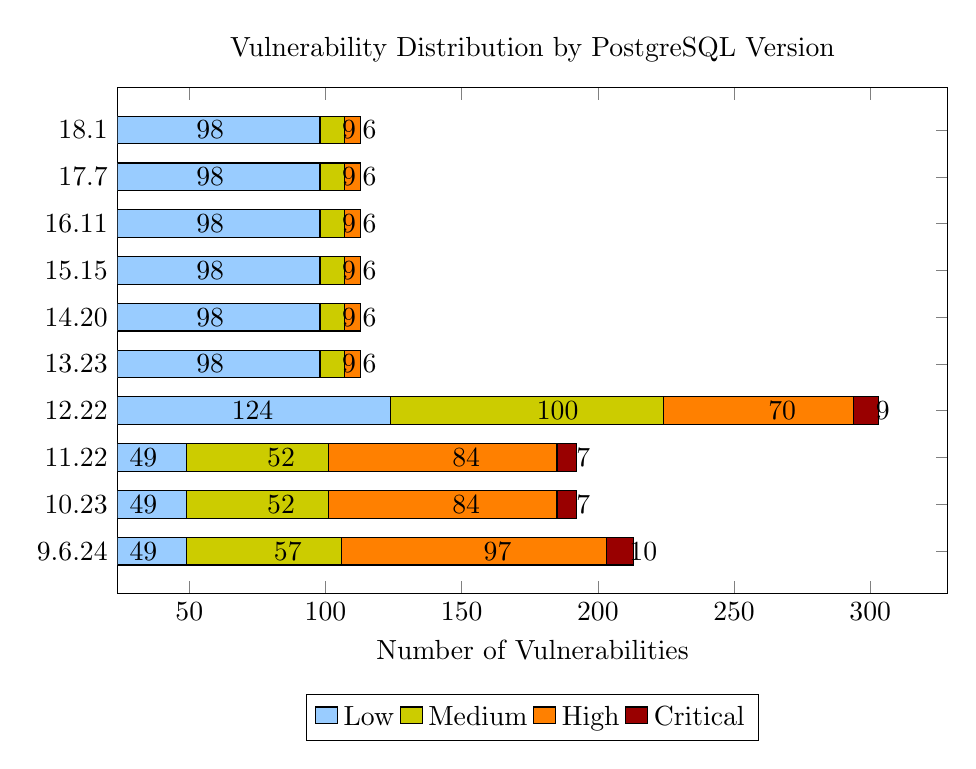
\begin{tikzpicture}
\begin{axis}[
    xbar stacked,
    width=\textwidth,
    height=8cm,
    title={Vulnerability Distribution by PostgreSQL Version},
    xlabel={Number of Vulnerabilities},
    symbolic y coords={9.6.24, 10.23, 11.22, 12.22, 13.23, 14.20, 15.15, 16.11, 17.7, 18.1},
    ytick=data,
    nodes near coords,
    nodes near coords align={horizontal},
    every node near coords/.style={
        font=\tiny,
        color=black,
        /pgf/number format/precision=0,
        /pgf/number format/fixed,
        /pgf/number format/zerofill=false
    },
    legend style={at={(0.5,-0.2)}, anchor=north, legend columns=-1}
]
\addplot[fill=vuln-low] coordinates {(98,18.1) (98,17.7) (98,16.11) (98,15.15) (98,14.20) (98,13.23) (124,12.22) (49,11.22) (49,10.23) (49,9.6.24)};
\addplot[fill=vuln-medium] coordinates {(9,18.1) (9,17.7) (9,16.11) (9,15.15) (9,14.20) (9,13.23) (100,12.22) (52,11.22) (52,10.23) (57,9.6.24)};
\addplot[fill=vuln-high] coordinates {(6,18.1) (6,17.7) (6,16.11) (6,15.15) (6,14.20) (6,13.23) (70,12.22) (84,11.22) (84,10.23) (97,9.6.24)};
\addplot[fill=vuln-critical] coordinates {(0,18.1) (0,17.7) (0,16.11) (0,15.15) (0,14.20) (0,13.23) (9,12.22) (7,11.22) (7,10.23) (10,9.6.24)};
\legend{Low, Medium, High, Critical}
\end{axis}
\end{tikzpicture}
\caption{Comparison of vulnerabilities detected by \texttt{trivy}.}
\label{fig:vuln-chart}
\end{figure}


\section{PostgreSQL Overview}

PostgreSQL \href{https://www.postgresql.org/}{https://www.postgresql.org/}, also known as Postgres, is a free and open-source relational database management system (RDBMS) emphasizing extensibility and technical standards compliance.

Postgres recommends that all users run the latest available minor release for whatever major version is in use.

The PostgreSQL Global Development Group supports a major version for 5 years after its initial release. After its five-year anniversary, a major version will have one last minor release containing any fixes and will be considered end-of-life (EOL) and no longer supported.

The Release roadmap \href{https://www.postgresql.org/developer/roadmap/}{https://www.postgresql.org/developer/roadmap/} lists upcoming minor and major releases. If the release team determines that a critical bug or security fix is too important to wait until the regularly scheduled minor release, it may make a release available outside the minor release roadmap.

A Feature Matrix \href{https://www.postgresql.org/about/featurematrix/}{https://www.postgresql.org/about/featurematrix/} documents feature availability against major releases.

\section{Summary and conclusion}

The combined data analysis is clear. Figure \ref{fig:vuln-chart} strikingly illustrates this divergence:

\begin{itemize}
    \item \textbf{The danger of unsupported versions:} Versions that have reached their end of life (12, 11, 10, 9.6) accumulate a dangerous number of vulnerabilities, including several \textbf{critical} ones.
    \item \textbf{The security of supported versions:} In contrast, images of maintained versions (14 to 18) show no critical vulnerabilities and a low, consistent risk profile. Note that PostgreSQL 13 is now unsupported.
    \item \textbf{Recommendation:} The choice of PostgreSQL version must be for an actively supported version. The security risk of using an obsolete version is real and high.\\
\end{itemize}

Tools like \texttt{geol} and \texttt{trivy} are essential in a modern DevSecOps approach. This analysis of PostgreSQL perfectly illustrates how abandoning software support directly leads to a drastic increase in security flaws. Using up-to-date versions is not just a recommendation, but a necessity for the security of any infrastructure.

\section{Resources}

\begin{itemize}
    \item \href{https://dev.to/adriens/geol-the-cli-to-efficiently-manage-eols-like-a-boss-3hne}{geol, the cli to efficiently manage EOLs like a boss}
    \item \href{https://youtu.be/ZqiXogK2fSw}{geol - Gérer la fin de vie (notebookLM slideshow) v1.3.0 - "for dummies" edition}
    \item \href{https://youtu.be/yCZRgAiQt9s}{geol 1.3.0 unboxing - the check command}
    \item \href{https://youtu.be/vhFXWGqB_-g}{MVP Unboxing geol - a devops secops cli to manage EOLs and product lifecycle}
    \item \href{https://github.com/adriens/geol-showcase}{geol-showcase, A set of resources to showcase what could be achieved with geol, datascience, AI and devsecops tools}
    \item \href{https://www.postgresql.org/about/news/postgresql-181-177-1611-1515-1420-and-1323-released-3171/}{PostgreSQL 18.1, 17.7, 16.11, 15.15, 14.20, and 13.23 Released!}
    \item \href{https://endoflife.date/postgresql}{PostgreSQL EOL Data}
\end{itemize}

\end{document}
